\section{Magnetoquasistatic Analysis}
In the frequency domain the used equations look like 
\begin{equation*}
	\nabla \times \vec{E} = -j\omega\mu\underline{\vec{H}}
	\hspace{1.6cm}
	\nabla \times \vec{H} = \vec{J} + j\omega \varepsilon \vec{E}
\end{equation*}
Since $\mu$ is much higher than $\varepsilon$, the term $j\omega\mu$ is dominant for smaller frequency. Therefor, $\frac{\partial \vec{D}}{\partial t} \approx 0$ which means thath the induced magnetic field due to the displacement current can be neglected (coupling only in one direction $\vec{B} \rightarrow \vec{E}$) which leads to the following equations in time domain
\begin{equation*}
	\nabla \times \vec{E} = -\frac{\partial \vec{B}}{\partial t}
	\hspace{2cm}
	\nabla \times \vec{H} = \vec{J}
	\hspace{2cm}
	\nabla \cdot \vec{B} = 0.
\end{equation*}
Since the divergence of the magnetic flux density is always equal to zero, the B-field can be described as
\begin{equation*}
	\vec{B} = \nabla \times \vec{A}
\end{equation*}
which leads to 
\begin{equation*}
	\nabla \times \left(\frac{1}{\mu} \nabla \times \vec{A}\right) = \vec{J} = \underbrace{\vec{J}_s}_{\textrm{source current density}} + \sigma \vec{E}.
\end{equation*}
With $\vec{E} = - \frac{\partial \vec{A}}{\partial t}$ this can be further simplified to
\begin{equation*}
	\nabla \times \left(\frac{1}{\mu}\nabla \times \vec{A}\right) + \underbrace{\sigma \frac{\partial \vec{A}}{\partial t}}_{\textrm{eddy currents}} = \vec{J}_s
\end{equation*}
If the material is homogeneous this equation can be written in time or frequency domain as 
\begin{equation*}
	\Delta\vec{A} -\mu\sigma\frac{\partial \vec{A}}{\partial t} = -\mu \vec{J}_s, (x,y,z)\in \Omega
	\hspace{2cm}
	\Delta\underline{\vec{A}} - j\omega\mu\sigma\underline{\vec{A}} = -\mu\underline{\vec{J}_s}, (x,y,z)\in \Omega
\end{equation*}

To solve a eddy current problem, first the initial current distribution $J_s$ needs to be computed if it is not given. The resulting total current density is then determined by:

\begin{equation*}
	\underline{\vec{J}} = \underline{\vec{J}_s} + \sigma\underline{\vec{E}} = \underline{\vec{J}_s} - j \omega \underline{\vec{A}} 
\end{equation*}

\textbf{\\ Boundary Value Problem (BVP)\\}
\begin{minipage}[lt]{11cm}
	\begin{tabular}{l}
		Magnetic insulation: \\
		\(\displaystyle n \times \vec{A} = 0,(x,y,z)\in \partial_D\Omega\)\\
		Boundary between to materials: \\
		\(\displaystyle n \times \vec{A}_1 = n \times \vec{A}_2), (x,y,z) \in \partial_N\Omega \) \\
		BVP (right example): \\
		\(\displaystyle \underline{A}_z = 0, \mathrm{ on } \partial_D\Omega \) \\
		\(\displaystyle \frac{\partial \underline{A}_z}{\partial n} = 0, \textrm{ o n} \partial_N\Omega \)
	\end{tabular}
\end{minipage}
\begin{minipage}[rt]{8cm}
	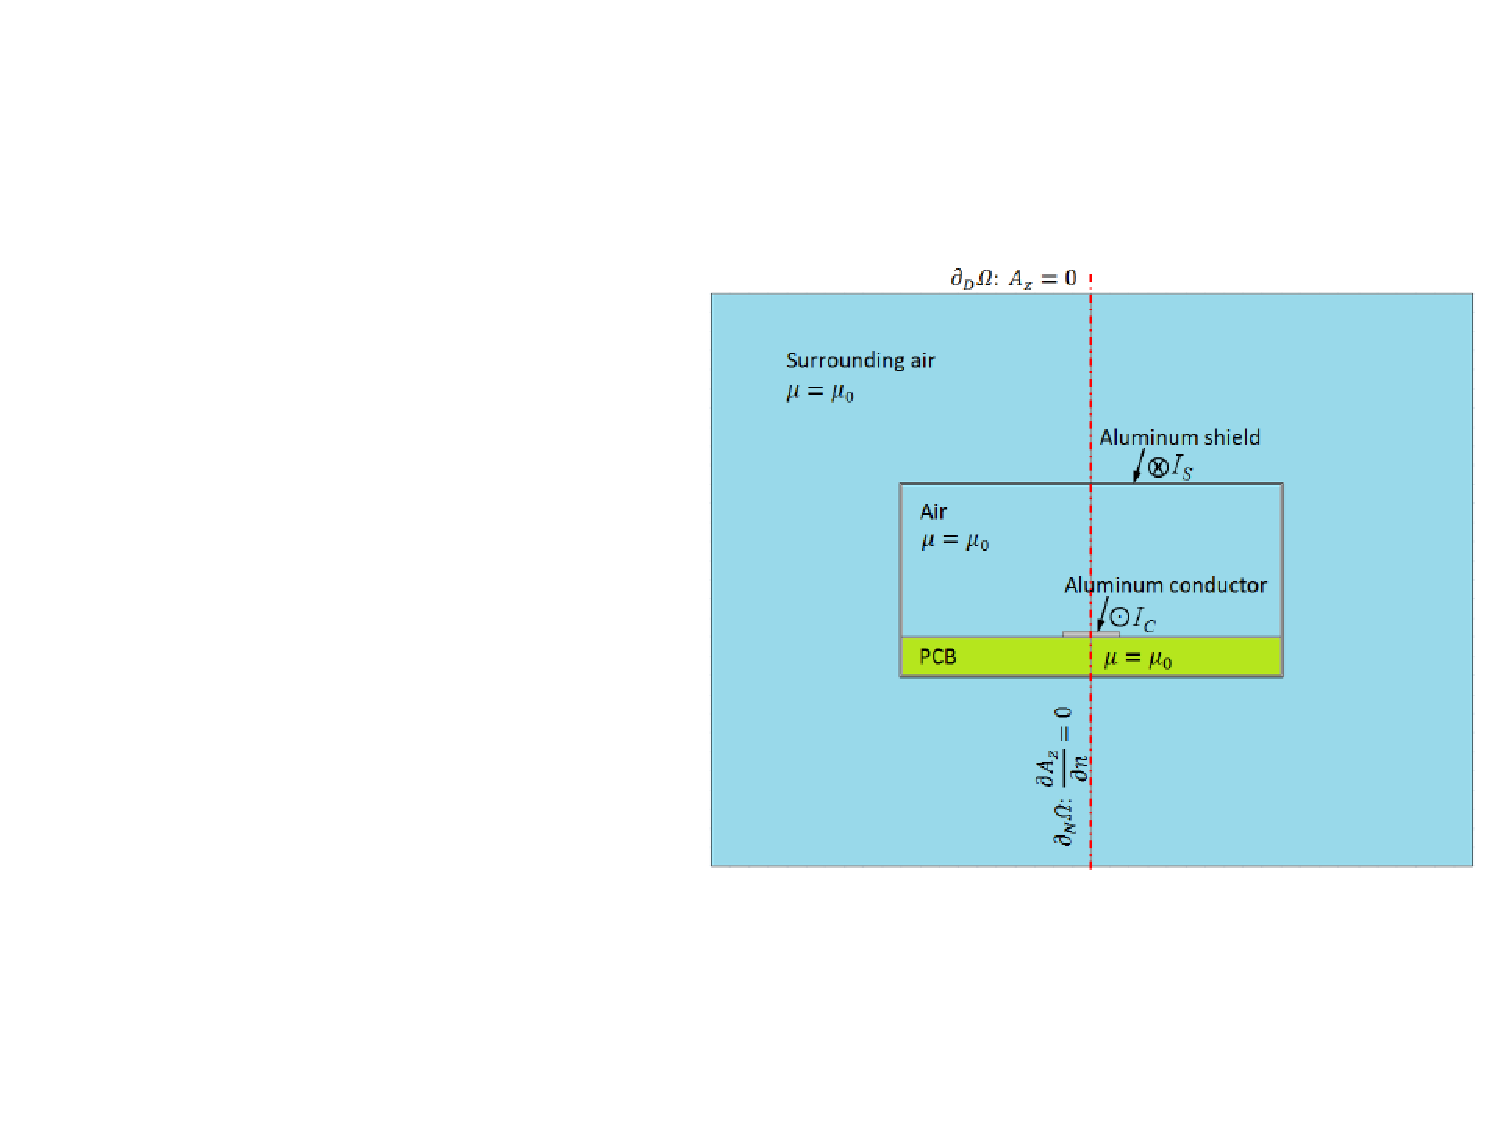
\includegraphics[width=.8\textwidth]{./images/BVP_magnetosquasistatic.pdf}
\end{minipage}